% Annual Cognitive Science Conference

\documentclass[10pt,letterpaper]{article}

\usepackage{cogsci}
\usepackage{pslatex}
\usepackage[natbibapa]{apacite}
\usepackage{graphicx}
\usepackage{floatrow}
\usepackage[fleqn]{amsmath}
\usepackage{amssymb}
\usepackage[longnamesfirst]{natbib}
\usepackage{url}

\renewcommand{\bibfont}{\small}
\renewcommand\bibsection{%
  \section*{\refname\markboth{\MakeUppercase{\refname}}{\MakeUppercase{\refname}}}%
  \addcontentsline{toc}{section}{\refname}%
}


\title{Representing and Learning a Large System of Concepts\\with Latent Predicate Networks}

\author{
  {\large \bf Joshua Rule, Eyal Dechter, Joshua B. Tenenbaum: $\{$rule, edechter, jbt$\}$ @ mit.edu}\\
%  {\large \bf Eyal Dechter (edechter@mit.edu)}\\
%  {\large \bf Joshua B. Tenenbaum (jbt@mit.edu)}\\
  MIT, 46-4053, 77 Massachussetts Avenue, Cambridge, MA 02139 USA}

\begin{document}

\maketitle

\begin{abstract}
  Conventional models of exemplar or rule-based concept learning tend
  to focus on the acquisition of one concept at a time. They tend to
  underemphasize the fact that we learn many concepts as part of large
  systems rather than as isolated individuals. In such cases, the
  challenge of learning is not so much in providing stand-alone
  definitions, but in describing the richly structured relations
  between concepts. The natural numbers are one of the first such
  abstract conceptual systems children acquire, serving as a serious
  case study in concept representation and acquisition
  \citep{fuson1988children,galGel2005,Car2009}. Even so, models of
  natural number learning focused on single-concept acquisition have
  largely ignored two challenges related to natural number's status as
  a \emph{system} of concepts: 1) there is an unbounded set of exact
  number concepts, each with distinct semantic content; and 2) people
  can reason flexibly about any of these concepts (even fictitious
  ones like \emph{eighteen-gazillion and thirty-one}). To succeed,
  models must instead learn the structure of the entire infinite set
  of number concepts, focusing on how relationships between numbers
  support reference and generalization.  Here, we suggest that the
  latent predicate network (LPN) -- a probabilistic context-sensitive
  grammar formalism -- facilitates tractable learning and reasoning
  for natural number concepts \citep{DecRulTen2015}. We show how the
  number words and their relations to one another can be expressed in
  this formalism and discuss a Bayesian learning algorithm for LPNs,
  suggesting a computational mechanism by which children might learn
  abstract numerical knowledge from linguistic utterances about
  numbers.

  \textbf{Keywords:}
  child development; concept learning; number; generalization;
  computational model; grammar induction;
\end{abstract}

\section{Introduction}

Humans seldom learn concepts in isolation. We learn about left by
comparing and contrasting it with up, down, and right, and about red
by noting its similarities and differences with green and blue. The
natural numbers (1, 2, 3, $\ldots$) are no exception: to understand a
number such as \emph{one}, we must not only ground it in terms of
concepts and percepts we already know, but we must also relate it to
other number concepts we are still in the process of acquiring. The
natural numbers are in fact particularly interesting in this respect.
Because they are infinite, there is no way to learn all the individual
concepts without learning the structure of the entire system.

A great deal of empirical work has focused on the first part of this
problem, on how initial number concepts are grounded in counting
routines and the core systems of approximate magnitude and parallel
object individuation
\citep{Car2009,dehaene2011number,feigenson2004core}. Recent studies
have also proposed computational mechanisms to explain several key
behavioral changes during early number learning
\citep{PianGoodTen2012}.

Far fewer studies have focused on the second half of the problem, on
how concepts are learned as systems and partially defined with respect
to each other. While the problems of how children link physical sets
with the counting routine and develop their first number concepts are
crucial, we direct our attention elsewhere in this paper. We focus on
this second problem, on how children might acquire knowledge of an
infinite number system, particularly for numbers they are unlikely to
ever see counted out explicitly.

Our approach shares much in common with the recent family of Rational
Rules models
\citep{goodman2008rational,T.D.Ullman:2012:1b1b6,PianGoodTen2012},
exploring concept learning through Bayesian induction of compositional
representations using sparse evidence. We agree that these points are
fundamental to understanding concept learning.

The major difference is in how our models represent concepts. In
Rational Rules models, each concept is a single stand-alone rule
supported by its own evidence. These rules are generated from a static
grammar which defines the hypothesis space. Learning is determining
which concepts (which rules) are supported by the evidence. In the
model we present here, concepts are not stand-alone rules, but
networks of possible relations generated according to a grammar. The
hypothesis space is thus not over stand-alone rules generated by a
pre-specified grammar, but over millions of possible grammars, each
defining a different network of relations. Learning is determining
which grammar, which sets of relations, are supported by the evidence.

We begin by discussing how to represent the infinite conceptual system
of natural number, and show how a particular formalism -- the
Probabilistic Range Concatenation Grammar (PRCG) -- can represent
number this way \citep{boullier2005range}. We then show how a portion
of this grammar can be learned using Bayesian inference in an LPN, a
learning framework for PRCGs \citep{DecRulTen2015}..

\section{Representing Number Knowledge}

To show how a system of concepts like number might be learned, we must
first understand what that system is and how it might be represented.
This task is non-trivial for number, and several models have been
proposed. For example, \citeauthor{hurford1975linguistic}
(\citeyear{hurford1975linguistic}) describes a single system
differentiating primitive and compound number concepts, while
\citeauthor{siegler1982development}
(\citeyear{siegler1982development}) propose a system with several
stages of development, each containing minimal internal structure.

To motivate our stance on the issue, we first describe several
challenges a representation of number must overcome. Finally, we show
how PRCGs, initially developed to explain context-sensitive syntactic
structures in natural language, can explain the conceptual structure
of number words.

\subsection{The Challenges of Number}

Relative to many other semantic fields children encounter ({\it e.g.}
color, kinship), natural numbers are highly distinctive.


First , there are infinitely many number concepts. While the
collection of, say, colors anyone might be able to name is fairly
small, there are an infinite number of readily-identified natural
number concepts. Being infinite, the amount of explicitly counted,
perceptually-grounded evidence children receive relative to the size
of the semantic field is incredibly sparse (When did you last see
exactly 253 objects?). In order to accommodate such an expressive
conceptual system in a finite mind, the concepts themselves must be
constructed as needed in a systematic and compositional manner.

Second, where many semantic fields refer to relatively concrete
classes of objects or object parts, the natural numbers refer
primarily to an abstract property (cardinality) of an abstract entity
(sets). Moreover, where many semantic fields are highly limited in
scope, natural number is incredibly broad, applying not only to
concrete objects, but also to things like sets ({\it e.g.} three pairs
of socks), sounds, events, time periods, people and other agents, and
numbers themselves ({\it e.g.} three threes makes nine). Being
infinite and broadly applicable suggests that numbers must be learned,
represented, and understood without direct perceptual grounding.

Third, numbers cannot be understood in isolation. Even when numbers
are used to describe cardinalities- as opposed to ordinals or
sequences -- interest may not be so much in the cardinality itself as
in some more complex property, such as whether it is more or less than
another cardinality or how it operates in arithmetic. Children may
eventually learn about negative and rational numbers, algebra,
geometry, and myriad other mathematical disciplines. This hugely
diverse range of meanings makes it impossible to fully describe
\emph{three} without referencing \emph{two}, \emph{four}, and
eventually all other numbers. The concept of \emph{two} (or any other
number) is not rightly understood as a single object, but must also
include the web of relationships in which \emph{two} participates.

How can we hope to represent systems of concepts which are: 1)
learnable without direct perceptual grounding; 2) compositionally
constructed; and 3) relationally defined? Happily, these properties
are similar to those linguists face in studying natural language
syntax. Motivated by this similarity, we use a grammar to represent
the system of natural number concepts. Grammars can be induced
directly from a stream of utterances, are highly compositional, and
define their constituents based on their relationships to each other
rather than as discrete objects.

\subsection{A Grammar for Number Concepts}

\begin{figure*}[t]
  \begin{centering}
    \includegraphics[width=\linewidth]{grammarOfNumber/gon.pdf}
    \caption{An RCG whose strings are valid number words. Numbered rules correspond to Figure \ref{fig:parse}.}
    \label{fig:gon}
  \end{centering}
\end{figure*}

\begin{figure*}[t]
  \begin{centering}
    \includegraphics[width=\linewidth]{parseTrees/parse.pdf}
    \caption{RCG parses for \emph{Number} (Blue) and \emph{Successor} (Red).}
    \label{fig:parse}
  \end{centering}
\end{figure*}

Having motivated our decision to model concepts as sets of grammatical
relations, we now present a grammar of number knowledge we have
constructed, capturing five key number relations: \emph{Number},
capturing the distinction between valid and invalid number words;
\emph{Succ} and \emph{Pred}, the successor and predecessor relations,
respectively; and \emph{More} and \emph{Less}, the more-than and
less-than relations, respectively. While seemingly basic tasks,
children require years to master them \citep{FusRicBriar1982}. While
most work in natural language syntax uses context-free grammars, our
focus on capturing structural relationships between concepts demands
that we use a context-sensitive grammar. We specifically use PRCGs
because they are expressive and context-sensitive while remaining
relatively tractable \citep{boullier2005range}.

Capturing these relations with an RCG is not only possible but can
be done quite compactly. Our grammar for the concepts of
\emph{Number}, \emph{Successor}, \emph{Predecessor}, \emph{Less}, and
\emph{More} covers all numbers between 0 and 1 billion, exclusive, and
requires only 216 rules. Even considering just \emph{Number},
\emph{Successor}, and \emph{Predecessor}, these 216 rules cover more
than 500 quadrillion relations. Figure \ref{fig:gon} shows a schematic
of the rules concerned with determining valid and invalid numbers,
while the rest, due to space constraints, can be found
online.\footnote{http://github.com/joshrule/GrammarInduction}

Two notes of clarification: First, our grammar never produces nor
parses full English sentences. This is a grammar for the structure of
concepts, not the structure of language. When attempting to parse
something like \emph{Succ(ninety nine, one hundred)}, we assume
another system more directly involved in language preprocesses
utterances into predicates which are then checked against the
knowledge encoded in our conceptual grammar. Second, this grammar has
not been optimized for compactness or efficiency. Implementing
\emph{More} with as the transitive closure of \emph{Successor}, for
example, would eliminate several predicates. We focused on providing a
grammar that would be correct, human-readable, and fit a
prefix-base-suffix understanding of number, as discussed below.

Intuitively, a number word like \emph{six-hundred thirty-seven} is
valid because we have six units of one hundred each and thirty-seven
remaining units of one each. That is, we have some base unit (hundred)
and we track both how many of them we have (six), and how many of the
next smallest base unit (one) we have (thirty-seven). We denote the
sum of these (six-hundred + thirty-seven) simply by concatenating the
two terms from largest to smallest base (six-hundred thirty-seven).
This structure is recursive. \emph{Nine-thousand seven-hundred
  sixteen} is created by taking nine thousands units and tacking on a
remainder, which is seven hundreds plus its remainder of sixteen ones:
\emph{nine} $\times$ \emph{thousand} $+$ (\emph{seven} $\times$
\emph{hundred} + (\emph{sixteen} $\times$ \emph{one})). Note that
there is no explicit mention of the base \emph{one} in a valid number
word - it is implied and marked by appending $\varnothing$, the empty
string, instead of \emph{one}.

Our grammar similarly uses a prefix-base-suffix system, and Figure
\ref{fig:parse} shows the concepts involved in deciding that
\emph{six-hundred thirty-seven} is a valid number word. As in our
example above, we must show that \emph{six} is a valid prefix for
\emph{hundred} and \emph{thirty-seven} is a valid suffix or remainder:
\setlength{\jot}{0pt}
\begin{align}
  & \textit{Number}(\textit{six hundred thirty seven}) \leftarrow\\
  & \textit{Prefix}(\textit{six}, \textit{hundred}), \textit{Suffix}(\textit{hundred}, \textit{thirty seven}).\notag
\end{align}

\noindent\emph{Six} is a valid prefix for \emph{hundred} because it is
a number word representing a \emph{ones} number, a number between one
and nine. It would be incorrect for \emph{hundred} to have no prefix,
and it would also be incorrect to use a prefix larger than
\emph{nine}:
\begin{align}
  & \textit{Prefix}(\textit{six}, \textit{hundred}) \leftarrow \textit{Ones}(\textit{six}).
\end{align}

\noindent\emph{Thirty-seven} is a valid suffix because it is a valid
number for a previous base, in this case $\varnothing$, the ones base:
\begin{align}
  & \textit{Suffix}(\textit{hundred}, \textit{thirty seven}) \leftarrow\\
  & \textit{LargerBase}(\textit{hundred}, \varnothing), \textit{Number}(\textit{thirty seven}).\notag
\end{align}

\noindent and
\begin{align}
  \textit{LargerBase}(\textit{hundred}, \varnothing) \leftarrow \textit{PrevBase}(\textit{hundred}, \varnothing).
\end{align}

\noindent\emph{Thirty-seven} is one of these numbers because it is
merely the concatenation of a \emph{decade} word and a \emph{ones}
word:
\begin{align}
  & \textit{Number}(\textit{thirty seven}) \leftarrow\\
  & \textit{Prefix}(\textit{thirty seven}, \varnothing), \textit{Suffix}(\varnothing,\varnothing).\notag
\end{align}

\noindent and
\begin{align}
  & \textit{Prefix}(\textit{thirty seven}, \varnothing) \leftarrow\\
  & \textit{Decades}(\textit{thirty}), \textit{Ones}(\textit{seven}).\notag
\end{align}


\noindent The compositional use of simple predicates thus helps us
analyze the structure of a complex phrase like \emph{six hundred
  thirty seven} and show that while it is a valid number word,
\emph{hundred six seven thirty} is not. \emph{Successor} and
\emph{More} can similarly be encoded (Figure \ref{fig:parse}), while
\emph{Predecessor} and \emph{Less} can be encoded quite simply as
$\text{Less}(X,Y) \leftarrow \text{More}(Y,X)$ and $\text{Pred}(X,Y)
\leftarrow \text{Succ}(Y,X)$.

\section{Learning Number Knowledge}

How might children learn the knowledge about number that is captured
in the representation presented above? In this section, we present a
computational model of learning over PRCGs and take a first step
towards evaluating this model against the learning trajectories and
patterns of error reported in the literature on counting. 

Because the learning problem is computationally challenging and
because much of the focus in the literature on exact number knowledge
has been on counting, we restrict our experiments here to the
successor relation, and, in particular, to learning how to count from
one to a hundred. Several studies of children's learning trajectories
and patterns of errors when acquiring the count
sequence~\citep{FusRicBriar1982,miller1987counting}. Thus, the
acquisition of the count sequence provides an interesting domain in
which evaluate how well our model of learning PRCGs fits the empirical
data.

% Learning to count up to a hundred does not come easily. Studies of
% counting in children between three and six years of age suggest that
% although some children are able to count up to a hundred shortly
% before entering kindergarten, many have trouble with the task at least
% as late as first
% grade ~\citep{FusRicBriar1982,miller1987counting}. These studies identify qualities learning trajectories and patterns of errors that children make. As such, These studies suggest
% that children do not learn to count to a hundred by memorizing the
% sequence of numbers between one and a hundred. As might be expected of
% a system that will eventually be able to count to arbitrarily large
% numbers, learning to count to a hundred involves discovering the
% pattern that successive number words follow. 

% We will model this process of pattern discovery as probabilistic
% inference over RCGs and show that the generalization phenomena
% described in these studies is captured by this model. 

\subsection{Latent Predicate Networks}

%% \begin{figure}[t]
%%   \begin{centering}
%%     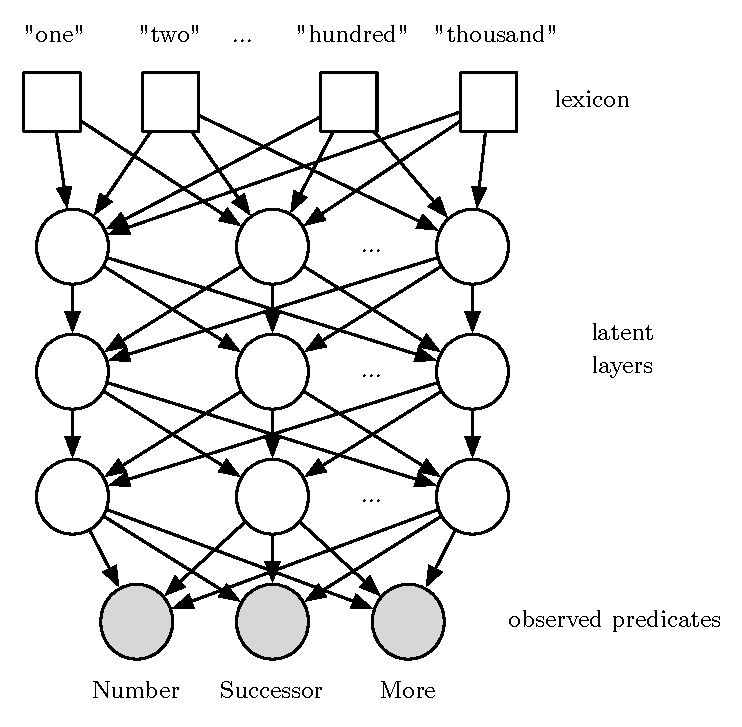
\includegraphics[width=0.9\linewidth]{lpn/lpn.pdf}
%%     \caption{A schematic LPN for number knowledge learning.}
%%   \end{centering}
%% \end{figure}

Latent Predicate Networks (LPNs) are PRCGs with a large number of
rules connected in a layered fashion. There are three types of
predicates in LPNs. The \emph{observed} predicates are relations that
are directly present in the data (e.g. the successor predicate Succ is
observed if the data is a collection of successor pairs). The observed
predicates are defined in terms of layers of \emph{latent}
predicates. These are relations that are not directly observable in
the data and whose meanings are determined through learning. For
example, the \emph{Decade} predicate, which is true for ``ten'',
``twenty'', etc., might correspond to one of the latent predicates
after the model is trained on pairs of successive number words. Each
layer of latent predicates is defined in terms of the latent predicate
layer beneath it, and the lowest layer of latent predicates is defined
in terms of a collection of \emph{lexicon} predicates, each of which
is a unary predicate that is true of the atomic units (the words) of
the system. The rules of the LPN consist all possible definitions
possible within the network architecture (for details see
~\cite{DecRulTen2015}), and the parameters of the network are the
probabilities of the rules.

Our model attempts to infer a distribution over the parameters of the
LPN given the data available to it. This inference is conducting via
hierarchical Bayesian inference~\citep{gelman2014bayesian}: the model
assumes that there is a prior distribution over the parameters of the
LPN and, using Bayes' rule, the model infers a distribution
over parameter values that balances the fit of the observations
against the prior. We use a sparsity inducing prior distribution which
formalizes the intuition that latent predicates and rules should be
shared in order to learn grammars that can generalize beyond the
observed data.

Exact inference in probabilistic grammars is computationally
intractable. We use the Variational Bayes EM algorithm~(CITATION), which has
been widely used in approximate inference of probabilistic context
free grammars~(CITATION). All the computations in this paper were done
using the PRISM probabilistic logic programming language~(CITATION).

All the simulations below were run on an LPN with three layers of five
predicates each. The learning algorithm was run for a single
iteration, a concentration parameter $\alpha=0.1$, and a convergence
criterion of $\epsilon=1e-4$. We will refer to each separate
simulation below as a \emph{simulated child}.

\subsection{Modeling the acquisition and elaboration of the count sequence}

\citet{FusRicBriar1982} describe qualitative phenomena of
count sequence acquisition and elaboration based on several surveys in
which they asked American children between three and five years of age
to count (either while counting a collection of objects or just
reciting the count world sequence). The learning trajectories and
error patterns they describe have inspired computation modeling
efforts using connectionist networks; for example,
\citet{ma1989modeling} use an associative network to model the errors
that young children typically make when learning the count sequence up
to twenty or thirty. But, to our knowledge, such models have not been
used to study how children acquire the count sequence beyond twenty.


\begin{figure*}[t]
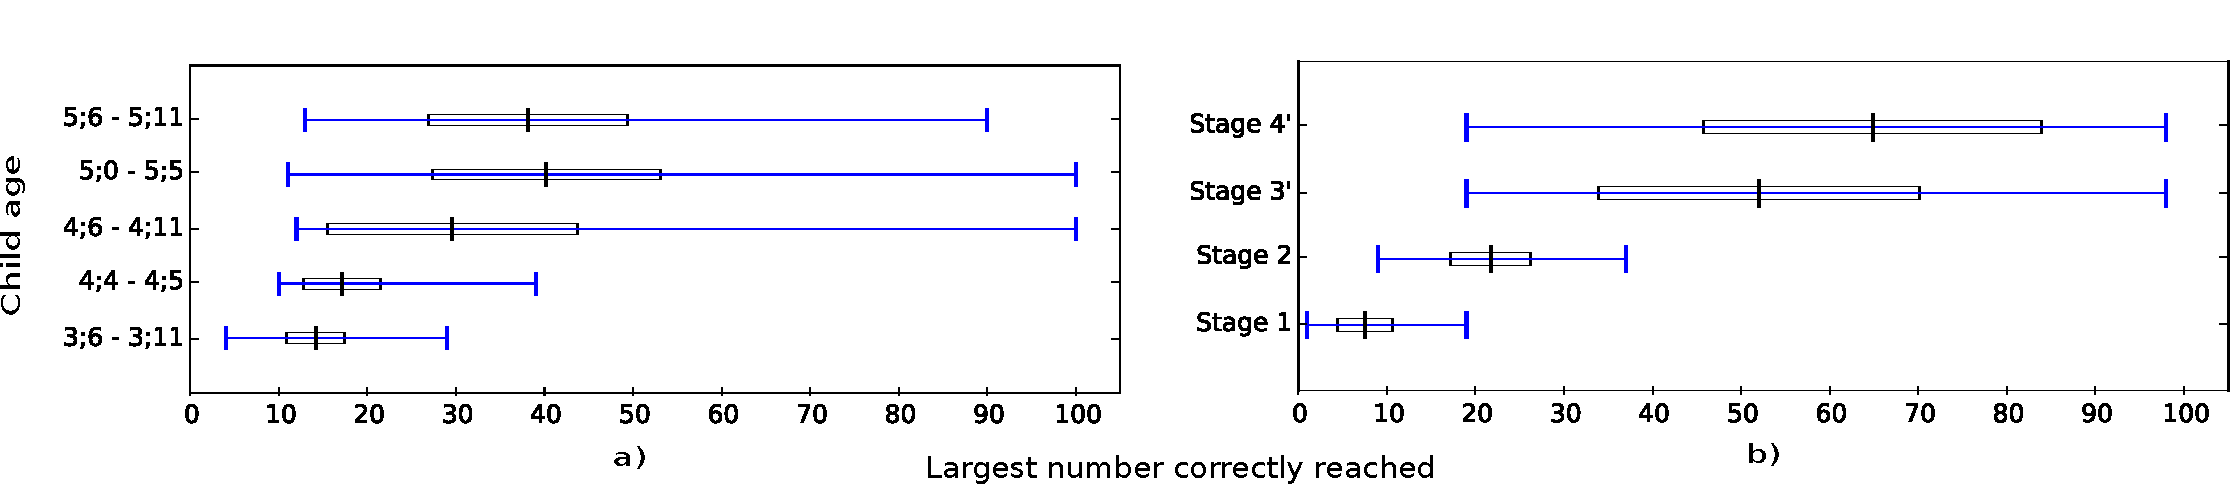
\includegraphics[width=0.7\linewidth]{figures/modelboxplot}
\caption{Our model compared with children's counting data a) Data
  from~\citet{FusRicBriar1982}. The x-axis shows the highest number
  correctly reached when children were asked to count starting at
  ``one.'' Boxes correspond to the standard deviation, central bands
  to the means, and whiskers to the range. b) Model performance,
  averaged over ten runs at four stages of increasing data quantity
  (see Figure~\ref{fig:counting_grid} for more detail). Whiskers
  correspond to the tenth and ninetieth percentiles.
\label{fig:fuson_model_comparison}}
\end{figure*}

Figure~\ref{fig:fuson_model_comparison}a shows the highest number
correctly reached by children in various age
ranges~\cite{FusRicBriar1982}. The authors hypothesize that the large
jump in range between the young three-year-olds and the older
four-year-olds and five-year-olds is due to the older children
partially solving what they term ``the decade problem.'' -- i.e.
recognizing both that there is a repetitive pattern of that repeats
across decades beyond twenty and learning that there is a particular
sequence to the decade words.

We asked whether our model goes through a similar transition. To
simulate learning, we generated data sets consisting of successor
pairs between one and a hundred, with the number of examples $N$ of each
pair $Succ(i+1, i)$ following the power law $N=\frac{K}{i}$, where $K$
determines the overall size of the data set. The explore the effect of
evidence quantity, and to simulate the effect that overall quantity
of evidence has on a child's acquisition of the count list, we
generated data sets for $K=10, 100, 1000, 10000$, which we denote
stages 1-4. The resulting histograms of data are shown in
Figure~\ref{fig:counting_grid}a-d (the y-axes are logarithmically
scaled).

For each of these data sets we ran our learning algorithm ten times,
generating ten simulated children at each stage (the simulations
differ due to different random parameter initializations). In
Figure~\ref{fig:counting_grid}a-d, each line corresponds to one of the
simulated children and shows the probability that the child will
correctly count to the corresponding number on the x-axis. To generate
this counting simulations, we asked the model for the distribution of
successors for a given number and used a simple soft max decision
procedure to determine the probability of the simulated child
reporting each word. Specifically, if the simulated child believes
that the $x$ follows $a$ with probability $p_a(x)$, then it says $x$
after $a$ for probability proportional to $p_a(x)^2 $.

The simulations in stage 1 are variable in their performances, with
some of simulated children unable to count further than the first few
words and a few having a relatively high chance of reaching
``twenty.'' The sharp drops in performance at the ``twenty,'' ``thirty''
and ``forty'' in stage 2, and the horizontal lines between them,
indicate that here the simulation has learned the within-decade
structure of the count list but is uncertain about the transitions
between decades. In stages 3 and 4, nearly all simulated children
master the numbers up to ``twenty nine'' but are unable to transition from
``thirty-nine'' to ``forty.'' And only in stage 4, do we see any
children making the transition from this state of knowledge to one in
which it can reach ``ninety nine.'' 

The simulations in these first four stages suggest that with even with
large increase in the quantity of data, the 1-to-29 counter mode is
likely to trap our model. We hypothesized that this is due to a lack
of evidence at the decade transitions. Mastering the decade
transitions requires both learning that there is a special rule for
the successor of numbers ending in ``nine,'' and learning the order of
decade words. This adds considerable complexity to the grammar, and
our simulations favor a more parsimonious explanation of the heavily
weighted smaller numbers. Children, however, do not learn to count to
a hundred by unsupervised exposure to naturally occurring count words;
they are actively taught to do so. Although we know of no study of the
pedagogical language used in teaching children to count, some kindergarten teaching
blogs\footnote{e.g. http://www.heidisongs.com/blog/2012/05/teaching-kids-to-count-to-100.html}
mention emphasizing decade transitions as useful in helping struggling
students to learn the count sequence.

To confirm that increased emphasis on decade transitions can
facilitate the transition to mastering counting up to a hundred, we
created two additional data sets, stages $3^*$ and $4^*$, that contain the
same data as stages 3 and 4, respectively, but have an additional
$10\%$ of the data evenly distributed across the decade transitions
(twenty nine, thirty; thirty nine, forty; ..., eighty-nine,
ninety). The simulated data for these stages is shown in
Figure~\ref{fig:counting_grid}e-f). In both simulations, we observe a
sharp increase in the number of simulated children who transition to
counting to a hundred (from zero to four in stage 3' and from two to
six in stage 4').



\begin{figure*}[t]
  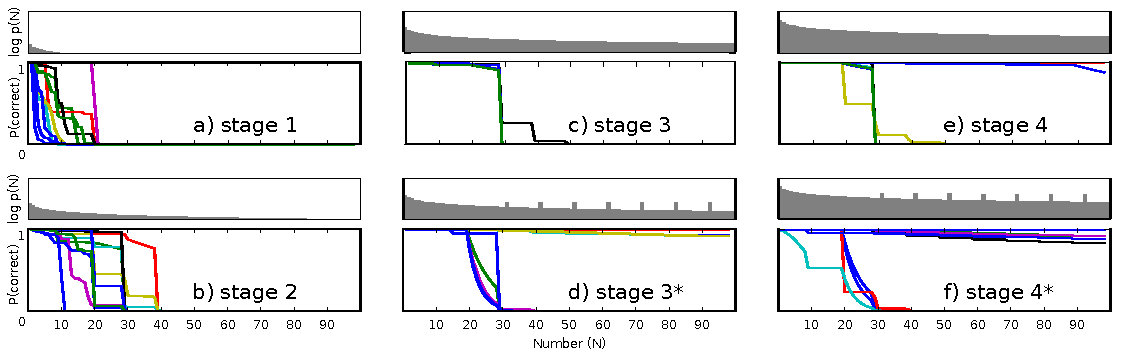
\includegraphics[width=\linewidth]{figures/counting_grid2}
  \caption{Our model's performance correctly reciting the count
    sequence. Each colored curve corresponds to a single run of the learning
    algorithm given the distribution of data in the histogram directly
    above it. For each number, $N$, along the x-axis, the y-axis
    corresponds to the probability that the model correctly counts
    from one up to $N$. The y-axes on the data histograms are shown on
    a logarithmic scale. The stages refer to the distributions of data
    available to the model (see text for details).
  }\label{fig:counting_grid}
\end{figure*}


Figure~\ref{fig:fuson_model_comparison}b summarizes the simulation
data for stages 1,2,$3^*$ and $4^*$ for comparison against the
\citeauthor{FusRicBriar1982} data in
Figure~\ref{fig:fuson_model_comparison}a. For each one of these stages
and for each simulated child, we computed the probability that highest
number counted starting at ``one'' would be $x$ for $x=1 \dots 98$. We
averaged these values across simulated children within a stage and
used the resulting densities to calculate the means, standard
deviations, and 10th and 90th percentiles for each stage (these
percentiles were chosen to be comparable with the empirical ranges described
by \citeauthor{FusRicBriar1982}

In addition to examining the learning trajectories of our model, we
also looked at the kinds of mistakes that it makes. One interesting
pattern of mistakes that young English speaking children make when
reciting the count sequence is that they invent number
words. \citeauthor{FusRicBriar1982} report that children invent such
words both by combining morphological components of number words (such
as ``fiveteen'' and ``eleventy'') and by combining decade words with
incorrect digit-place words (such as ``twenty-eleven'' and
``twenty-twenty''). In particular, they report that appending
\emph{teen} words to decade words is most common, creating sequences
like ``twenty-ten'', ``twenty-eleven'', ``twenty-twelve'', etc.
In Figure~\ref{fig:inventedWordComparison} we show the most common invented
words that \citeauthor{FusRicBriar1982} report and the mean number of
times each child in their study use the word. 

Since we do not model in this work the way in which the number word
morphemes are composed to construct number words, our model cannot
account for the morphologically based word errors. We asked, however,
to what extent it can model the other invented word errors that
\citeauthor{FusRicBriar1982} report; the most common invented words
are shown in Figure~\ref{fig:inventedWordComparison}a). To compare
these data to our model, we asked a stage 2 simulated child for the
top twenty non-number words that could appear as successor to a number
world or non-number word (because this was a computationally expensive
procedure, we restrict our analysis here to a single randomly selected
simulation). The marginal probabilities of those non-number words is
shown in Figure~\ref{fig:inventedWordComparison}.

There is evidence that there are cross-linguistic differences in the
kinds of errors that children make when learning the count sequence.
In their study comparing American and Chinese four to six-year-olds,
\citeauthor{miller1987counting} found that while $20\%$ of the errors
that English speaking children made involved invented numbers, they
encountered no instances of Chinese-speaking children doing so.


Our model agrees that Chinese children should use fewer invented
words: we simulated a stage 2 child using the Chinese number system
and found only a single invented word ``one ten one'' with marginal
probability $3e-4$, making it much less probable than the twenty most
probably invented words for the English speaking simulated child.  Our
model suggests that the reason the use of invented words is more
common in English than Chinese is because there are more categories of
words in the English system than the Chinese one. In Chinese, the
decade word are the same as the unit words (e.g. ``five-ten-one'' for
51) and the teen words (11-19) are uniform in contruction
(e.g. ``ten-five'' for 15). Thus, there are both fewer words to learn
about in the Chinese system, and grammar rules in the Chinese system
that combine words of different categories are far less likely to
produce invalid words than those in the English system.

Our model also is consistent with \citeauthor{miller1987counting}'s finding
that, contrary to their original expectations, Chinese children do not
count by decades (e.g. ``twenty nine'', ``thirty'', ``forty,'' ...)
more often than their English speaking counterparts. In our
simulations we do not find any suggestion of this kind of error for
the Chinese-speaking simulated children, and this is likely because
our grammar rules do not act independently on different parts of the
number words. The rules explicitly act on both categories of
substrings and their relative positions, so the use of a rule that
increments the units position of a number word does not increase the
probability of a rule that increments the decades position, even if
the those words happen to be the same.


% \begin{figure}[t]
% 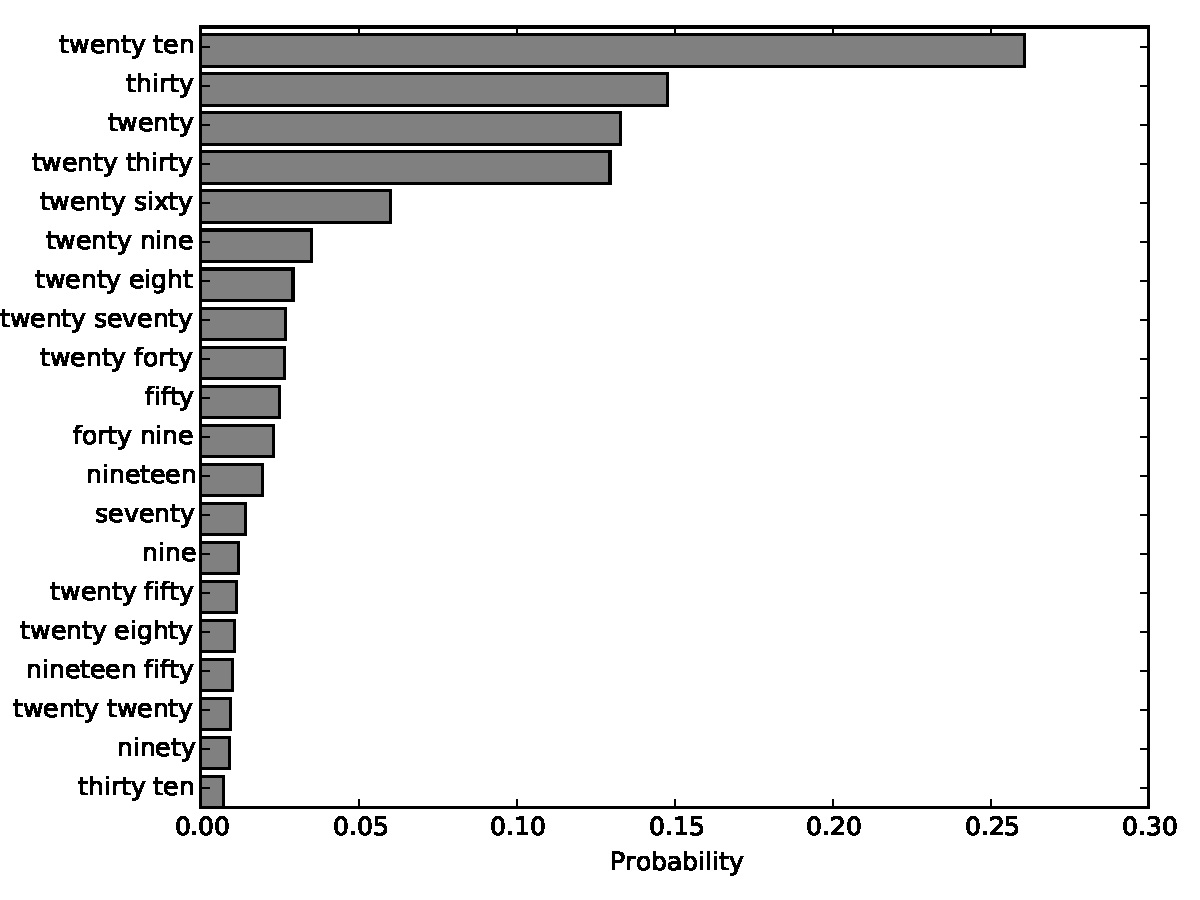
\includegraphics[width=0.9\linewidth]{figures/after29}
% \caption{The distribution over successors of ``twenty nine'' for
%   averaged over simulated children at stage 2.\label{fig:after29}}
% \end{figure}


\begin{figure}[t]
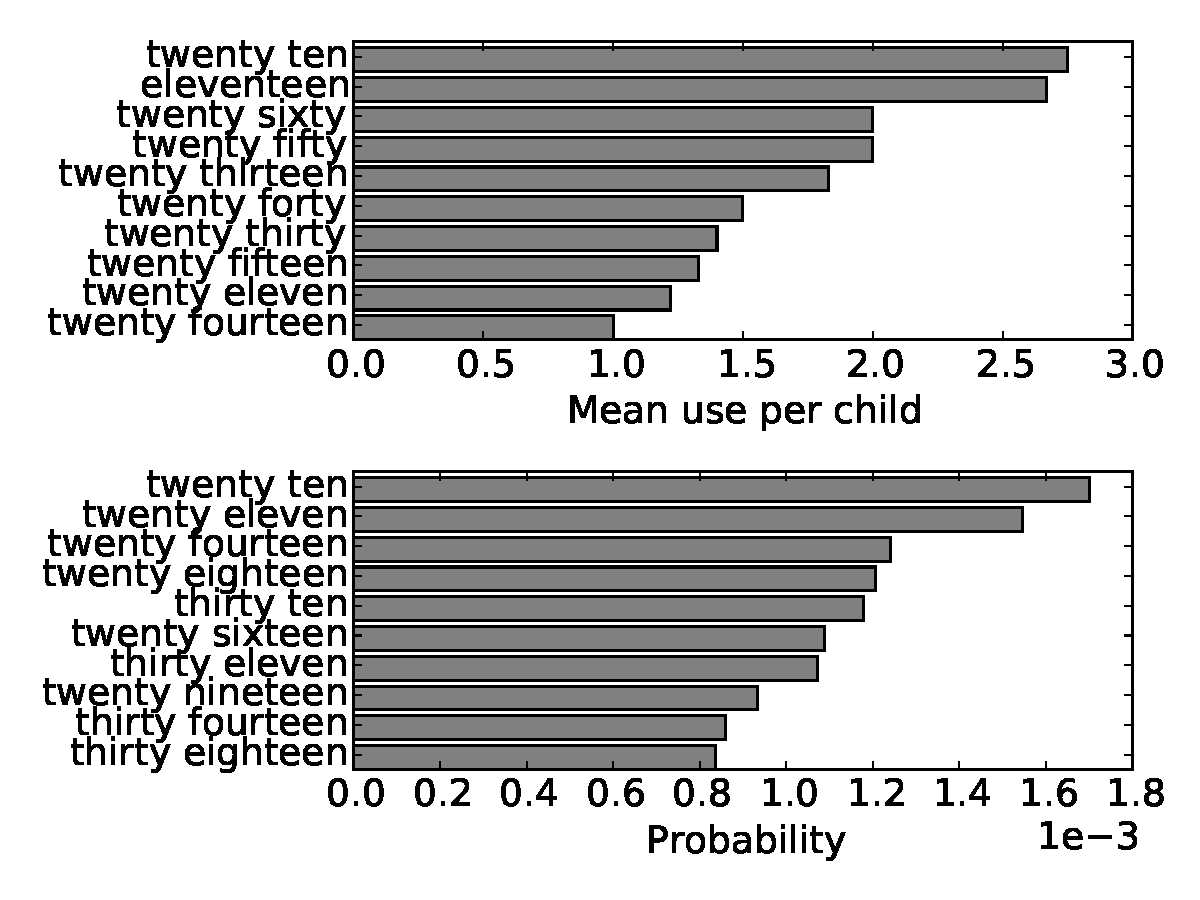
\includegraphics[width=0.9\linewidth]{figures/inventedWordComparison}
\caption{Top ten invented number words in children's counting. a) Data
  from \citeauthor{FusRicBriar1982} b) A simulated child at stage~2.
   \label{fig:inventedWordComparison}}
\end{figure}


\section{Discussion}

In this work, we have shown how the infinite set of exact number
concepts and the relations among them can be represented using
probabilistic context-sensitive grammars. We have also given a model
for how children might learn such representations based on
hierarchical Bayesian inference. Our simulations suggest this model
captures several behavioral phenomena children exhibit learning the count
sequence -- a critical and difficult prerequisite to adult-like
numerical knowledge.

An interesting aspect of this process is the seemingly sudden
transition from counting only through the first few decades to
counting all the way to a hundred. Our model explains this transition
as an inductive leap: for small amounts of data, learning is slow and
incremental -- adding a decade at a time -- because the increased
complexity of the conceptual knowledge is large compared to the gains
in explanatory power. Eventually, however, enough evidence accumulates
to warrant a more complex and more general grammar, resulting
in a kind of phase transition between states of knowledge.

In many ways this phenomenon is analogous to the Cardinal Principle
(CP) transition, in which younger children learning the relationship
between small numbers and set sizes make slow and incremental progress
when learning the meanings of the first three or four numbers but then
suddenly expand their understanding to the remaining numbers that
they know. The theory that this rapid transition is due to what Carey
(\citeyear{Car2009}) refers to as \emph{Quinian bootstrapping} has
been formalized by Piantadosi et al. (\citeyear{PianGoodTen2012}) as
probabilistic inference over a space of recursive programs defined by
a grammar. As we do here, they explain the inductive leap of the CP
transition as a result of the tension between program complexity and
fit to the available data. Crucially, whereas Piantodosi et al. place
a distribution over programs using a probabilistic context-free
grammar, our model here is learning a complete grammar, one that can
accommodate many different concepts and relations and that can be seen
as a probabilistic and declarative knowledge base.

Another difference is that our simulations require a pedagogical
emphasis on critical evidence -- the decade transitions -- to master
the count sequence robustly, suggesting that pedagogy may play an
important role in facilitating these kinds of inductive leaps.
Focusing on concept acquisition in slightly older children allows us
to explore the relationship between computational level considerations
driving inductive reasoning and the pedagogical factors enabling it in
practice.

An important future step for this research will be to relate our model
to those, like Piantadosi et al. (\citeyear{PianGoodTen2012}) for
counting and Dehaene et al. for the approximate magnitude system, that
attempt to explain how abstract number knowledge becomes grounded in
the perceptual and procedural primitives through which children learn
about the world. The model we presented here does not attempt to
explain how children come to understand that number words refer to
cardinalities, though this is crucial to understanding number.

That said, we see no fundamental incompatibility between the model
presented here and extensions to include approximate magnitude, object
tracking, set manipulation, more complex morphology ({\it e.g.} the
meaning of \emph{-illion} or \emph{-teen}), or different counting
strategies ({\it e.g.} as used in Turkish, French, or Mandarin) as
would be needed for a more comprehensive model of number learning. We
see our work here as a first demonstration of LPN's suitability for
capturing a broad range of concepts in number and other semantic
domains including space, kinship, and natural kinds.  Whether these
more general models are best approached by working strictly within the
LPN formalism or by using it as one module within a more complex
framework is an open question. Certainly, the human mind is more
powerful than an RCG and is at least Turing-complete.  RCGs provide a
tractable way, however, to explore a restricted subclass of
problems. The strategies and solutions we discover here are also
available in Turing-complete systems, and are in fact implemented in
one (PRISM Prolog), so our findings easily generalize to more
expressive grammars.

More broadly, we see this paper as growing out of the hypothesis that
much of human learning, including the explosion of knowledge during
development, can be understood as inducing, from sparse and noisy data,
a library of bits of conceptual knowledge, written in something like a
programming language of thought. This vision of the
\emph{child-as-hacker} draws on and extends the notion of the
\emph{child-as-scientist} \citep{gopnik1996scientist}; not only are
children forming theories about the world, but they are simultaneously
developing the very conceptual language they use to formulate those
theories.

%% \section{Acknowledgments}
%% 
%% The authors benefited significantly from conversations with Timothy
%% O'Donnell and Leon Bergen. This material is based upon work supported
%% by the Center for Minds, Brains and Machines (CBMM), funded by NSF STC
%% award CCF-1231216, an NSF Graduate Research Fellowship, and the Eugene
%% Stark Graduate Fellowship.


\bibliographystyle{apacite}

\setlength{\bibleftmargin}{.125in}
\setlength{\bibindent}{-\bibleftmargin}
\bibliography{cogsci}

\end{document}
